\begin{fact} \label{iso-rect}
	Considérons tous les rectangles de périmètre fixé $p$. Parmi tous ces rectangles, un seul est d'aire maximale, c'est le carré de côté $c = \num{.25} p$.
\end{fact}


\begin{proof}
	Voici une preuve géométrique élémentaire s'appuyant sur le dessin suivant où les rectangles $1$, $2$ et $3$ sont isométriques au rectangle vert étudié de dimension $L \times \ell$.

	\begin{center}
		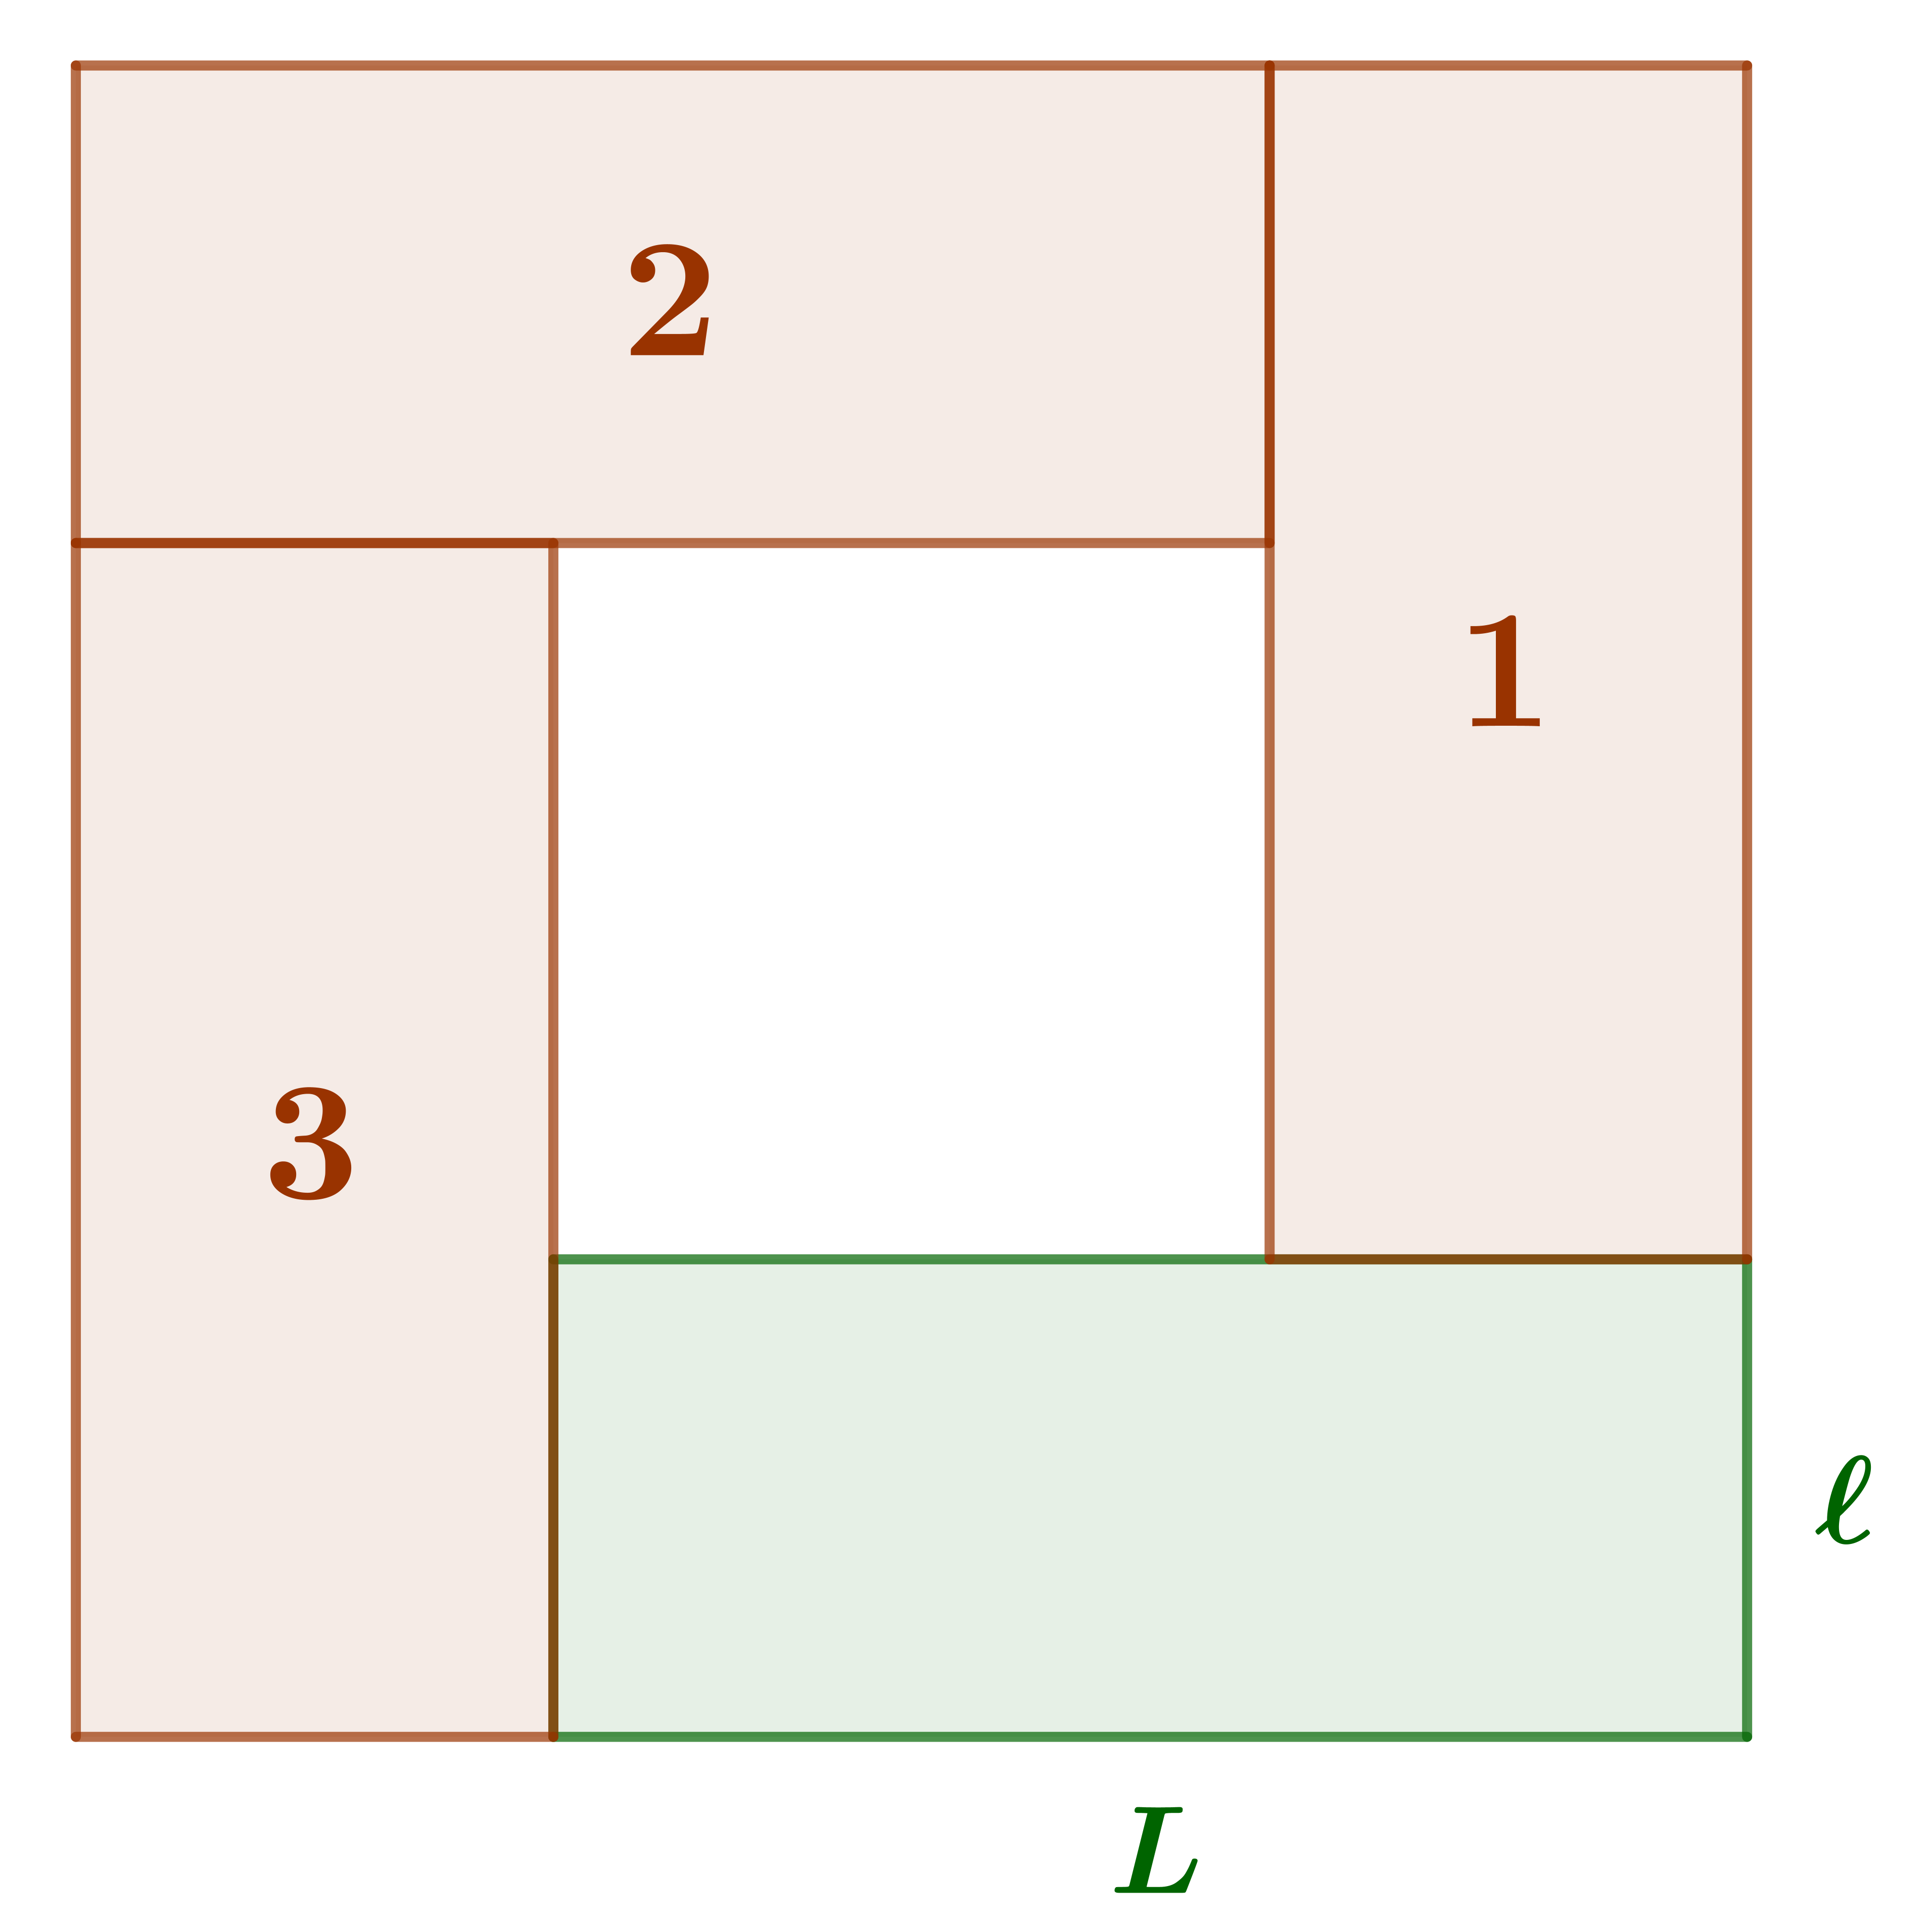
\includegraphics[scale=.4]{content/rectangle/rectangle.png}
	\end{center}
	
	Le raisonnement tient alors aux constations suivantes accessibles à un collégien.
	%
	\begin{enumerate}
		\item Le grand carré a une aire supérieure ou égale à $4 L \ell$, et même strictement si le rectangle initial n'est pas un carré.

		\item Le grand carré a un périmètre égal à $4 (L + \ell)$.

		\item Une homothétie de rapport \num{.5} donne un carré 
		de périmètre $\num{.5} \times 4 (L + \ell) = 2 (L + \ell)$,
		et d'aire supérieure ou égale à $\num{.5}^2 \times 4 L \ell =  L \ell$, avec inégalité stricte si le rectangle initial n'est pas un carré.
	\end{enumerate}
	
	Donc, parmi tous les rectangles de périmètre $p = 2 (L + \ell)$ et d'aire $L \ell$, le seul qui puisse avoir une aire maximale est le carré. Joli! Non?
\end{proof}


% ----------------------- %


\begin{remark}
	Une preuve courante est d'exprimer l'aire du rectangle comme un polynôme du 2\ieme\ degré en $L$ par exemple.
	On obtient $L \ell = L (\num{.5} p - L)$ qui est maximale en $L_M = \num{.25} p$ (moyenne des racines), d'où $\ell_M = \num{.25} p = L_M$.
\end{remark}


% ----------------------- %


\begin{remark}
	Au passage, nous avons pour $(L ; \ell) \in \big( \RRsp \big)^2$, $4 L \ell \leq (L + \ell)^2$, c'est-à-dire $2 L \ell \leq L^2 + \ell^2$, d'où $\sqrt{L \ell} \leq \sqrt{\frac12 (L^2 + \ell^2)}$, soit la comparaison des moyennes géométriques et quadratiques d'ordre $2$.
\end{remark}
